\documentclass[resume]{subfiles}


\begin{document}
\begin{multicols}{3}
\section{Opamp 3}
\subsection{Bruit}
$$\text{SNR}=\frac{S}{N}=\frac{\text{signal rms}}{\text{bruit rms}}$$
Le bruit est représenté par une gaussienne avec $\mu$ la moyenne et $\sigma$ l'écart-type
\paragraph{Somme de puissances de bruit (rms)}
$$\boxed{E_\text{tot}=\sqrt{e_1^2+e_2^2+e_3^2}}$$
\paragraph{Bruit dans une résistance}
$$U_R=\sqrt{4ktR}\quad\left[\frac{\si{\volt}_\text{rms}}{\sqrt{\si{\hertz}}}\right]$$
Entre deux fréquences on obtient
$$U_R=\sqrt{4ktR(f_{max}-f_{min})}\quad \left[\si{\volt_\text{rms}}\right]$$
Constante de Boltzmann :
$$k=\SI{1.38e-23}{\joule\per\kelvin}$$

\subsubsection{Densité spectrale de puissance du bruit}
La densité spéctrale de puissance est référencée sur une résistance de \SI{1}{\ohm} par défaut
$$\frac{\si{\volt}_\text{rms}}{\sqrt{\si{\hertz}}}\quad \text{ou}\quad \frac{\si{\ampere}_\text{rms}}{\sqrt{\si{\hertz}}}$$
\paragraph{Bruit blanc} : Constant sur toute la plage de fréquences
\paragraph{Densité de bruit} : Varie en fonction de la fréquence
\begin{figure}[H]
\centering
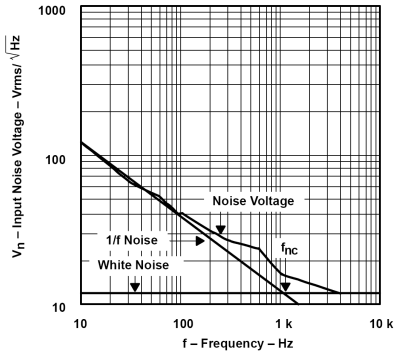
\includegraphics[width=6.00cm]{img_78.png}
\end{figure}
\paragraph{Calcul de la puissance de bruit entre $f_{min}$ et $f_{max}$}
$$E_n=E_{\text{white noise}}\sqrt{f_{nc}\ln\left(\frac{f_{max}}{f_{min}}+(f_{max}-f_{min}\right)}$$
\subsection{Calcul du bruit dans un circuit}
Convertir chaque source en trouvant de quoi la transformer le plus proche possible (résistance par exemple). On cherche à avoir tous les bruits au même endroit et avec la même unité
\begin{figure}[H]
\centering
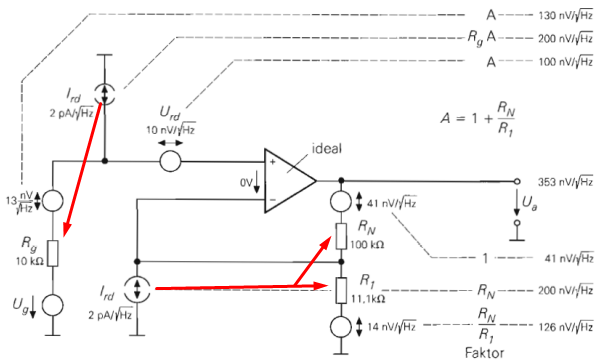
\includegraphics[width=0.9\columnwidth]{img_79.png}
\end{figure}
\subsection{Auto-zero}
Suppression du bruit à basse fréquence par mesure et soustraction de l'offset
\begin{figure}[H]
\centering
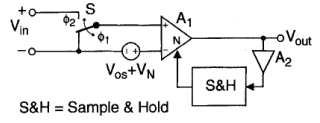
\includegraphics[width=5.00cm]{img_80.png}
\end{figure}
\begin{figure}[H]
\centering
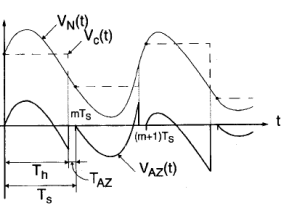
\includegraphics[width=5.00cm]{img_81.png}
\end{figure}
En circuit on obtient :
\begin{figure}[H]
\centering
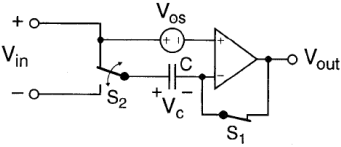
\includegraphics[width=5.00cm]{img_82.png}
\end{figure}
\subsection{Chopper amplifier}
Modulation du signal d'entrée par un carré à haute fréquence puis démodulation à la sortie. Le but est d'effectuer du "noise shaping" pour placer le bruit dans la zone qui va être supprimée.
\end{multicols}
\end{document}